\documentclass{PoS}

% Shortcuts
\newcommand{\aap}{AAP}
\newcommand{\pasp}{PASP}
\newcommand{\url}[1]{\href{#1}{#1}}

\title{Gammapy -- A prototype for the CTA science tools}
\ShortTitle{Gammapy -- A prototype for the CTA science tools}

\author{
Christoph Deil$^a$,
Roberta Zanin$^a$,
Julien Lefaucheur$^b$,
Catherine Boisson$^b$,
Bruno Kh\'elifi$^c$,
R\'egis Terrier$^c$,
Matthew Wood$^d$,
Lars Mohrmann$^e$,
Nachiketa Chakraborty$^a$,
Jason Watson$^a$,
Rub\'en L\'opez Coto$^a$,
Stefan Klepser$^f$,
\speaker{Matteo Cerruti}$^g$,
Jean-Philippe Lenain$^g$,
Fabio Acero$^h$,
Arache Djannati-Ata{\"\i}$^c$,
Santiago Pita$^c$,
Zeljka Bosnjak$^i$,
Jose Enrique Ruiz$^j$,
Cyril Trichard$^k$,
Thomas Vuillaume$^l$,
for the CTA Consortium,
Axel Donath$^a$,
Johannes King$^a$,
L\'ea Jouvin$^c$,
Ellis Owen$^m$,
Manuel Paz Arribas$^n$,
Brigitta Sipocz$^o$,
Dirk Lennarz$^p$,
Arjun Voruganti$^a$,
Marion Spir-Jacob$^c$
\\
\llap{$^a$}MPIK, Heidelberg, Germany\\
\llap{$^b$}LUTH, Obs. de Paris/Meudon, France\\
\llap{$^c$}APC/CNRS, Paris, France\\
\llap{$^d$}SLAC National Accelerator Laboratory, US\\
\llap{$^e$}FAU, Erlangen, Germany\\
\llap{$^f$}DESY, Zeuthen, Germany\\
\llap{$^g$}LPNHE, Paris, France\\
\llap{$^h$}CEA/IRFU, Saclay, France\\
\llap{$^i$}University of Rijeka, Croatia\\
\llap{$^j$}Instituto Astrof\'isica de Andaluc\'ia, Granada, Spain\\
\llap{$^k$}CPPM, Marseille, France\\
\llap{$^l$}LAPP, Annecy-le-Vieux, France\\
\llap{$^m$}UCL-MSSL, Dorking, United Kingdom\\
\llap{$^n$}Humboldt University, Berlin, Germany\\
\llap{$^o$}Cambridge, UK\\
\llap{$^p$}Georgia Tech, Atlanta, US\\
E-mail:
\email{Christoph.Deil@mpi-hd.mpg.de},
\email{Roberta.Zanin@mpi-hd.mpg.de},
\email{julien.lefaucheur@obspm.fr},
\email{catherine.boisson@obspm.fr},
\email{khelifi@apc.in2p3.fr},
}

\abstract{

Gammapy is a Python package for high-level gamma-ray data analysis built on
Numpy, Scipy and Astropy. Starting with event lists and instrument response
information, it is possible to analyse gamma-ray data and to create for example
sky images, spectra and lightcurves, and to determine the position, morphology
and spectra of gamma-ray sources.

So far Gammapy has mostly been used to analyse data from H.E.S.S. and Fermi-LAT,
and now it is being used for the simulation and analysis of observations from
the Cherenkov Telescope Array (CTA). We have proposed Gammapy as a prototype for
the CTA science tools. This contribution will give an overview of the Gammapy
package and show an analysis application example with simulated CTA data.

}

\FullConference{35th International Cosmic Ray Conference --- ICRC2017\\
		10--20 July, 2017\\
		Bexco, Busan, Korea}


\begin{document}

\section{Introduction}
\label{sec:intro}

% CTA science tools
The Cherenkov Telescope Array (CTA) will observe the sky in very-high-energy
gamma-ray light soon. All astronomers will have access to CTA high-level data,
as well as CTA science tools (ST) software. The ST can be used for example to
generate sky images and to measure source properties such as morphology, spectra
and light curves, using event lists as well as instrument response function
(IRF) and auxiliary information as input.

% What is Gammapy?
Gammapy is a prototype for the CTA ST, built on the scientific Python stack and
Astropy, optionally using Sherpa or other packages for modeling and fitting (see
Figure~\ref{fig:stack}). Initially the focus was to implement the ``classical
TeV analysis'', using 2-dimensional sky images for detection and morphology
characterization, followed by spectral analysis for a given source region. A
3-dimensional analysis with a simultaneous spatial and spectral models of the
gamma-ray emission, as well as background (called ``cube analysis'' in the
following) is in development. At the moment likelihood fitting in Gammapy is
done on binned data (images, spectra, cubes, lightcurves), unbinned likelihood
is not implemented. Simulating observations is done by Poisson-fluctuating
predicted counts according to given sky models, IRFs and observation parameters,
event samplers are not implemented. So far we have not encountered important use
cases that require an unbinned likelihood, but if needed for efficient analysis
of some use cases, a likelihood function using unbinned events or sparse or
multi-resolution maps could be added in the future.

% Existing studies using Gammapy
A first study comparing spectra obtained with the classical 1D analysis and the
3D cube analysis using point source observations with H.E.S.S., to compare the
methods and to validate Gammapy, is presented in \cite{lea}. Further
developments and verification using data from existing Cherenkov telescope
arrays such as H.E.S.S. and MAGIC, as well as simulated CTA data is ongoing.
% Gammapy use in CTA
Gammapy is starting to be used for scientific studies for existing ground-based
gamma-ray telescopes \cite{hgps, shells}, the Fermi-LAT space telescope
\cite{owen2015}, as well as for CTA \cite{julien, roberta, cyril}.

\section{Context}
\label{sec:context}

% Python, Numpy, Astropy
Before moving on to a description of Gammapy in the next section, we would like
to give some context for it's development and mention some related projects. An
early prototype package that was similar to Gammapy was ``PyFACT: Python and
FITS Analysis for Cherenkov Telescopes'' \cite{pyfact}. It was developed in
2011/2012 and hasn't been updated since, we mainly mention it to show that the
idea to build the CTA science tools as a Python package using Numpy. In 2011,
the Astronomical Python community came together and created the Astropy project
and package \cite{astropy}, which is a key factor making Python the most popular
language for astronomical research codes (at least according to this informal
survey \cite{momcheva2015}). Gammapy is an Astropy affiliated package, which
means that where possible it uses the Astropy core package instead of
duplicating it's functionality, as well as having a certain quality standard
such as having automated tests and documentation for the available
functionality. In recent years, several other packages have adopted the same
approach, to build on Python, Numpy and Astropy. To name just a few, there is
ctapipe (\url{https://github.com/cta-observatory/ctapipe}), the prototype for
the low-level CTA data processing pipeline (up to DL3); Naima for modeling the
non-thermal spectral energy distribution of astrophysical sources \cite{naima};
and PINT, a new software for high-precision pulsar timing
(\url{https://github.com/nanograv/PINT}), and Fermipy
(\url{https://github.com/fermipy/fermipy}), a Python package that facilitates
and analysis of data from the Large Area Telescope (LAT) with the Fermi Science
Tools and adds some extra functionality.

We note that many other astronomy projects have chosen Python/Astropy as the
basis both for their data calibration and reduction pipeline as well as the
science tools used by astronomers. Some prominent examples are the Hubble space
telescope (HST) (TODO: add reference), the upcoming James Webb Space Telescope
(JWST) (TODO: add reference) and the Chandra X-ray observatory \cite{chandra,
sherpa2001}. Even projects like LSST that started their analysis software
developments before Astropy existed and are based on C++/SWIG are now actively
looking for ways to collaborate and make their software stack interoperate with
Numpy and Astropy to avoid code duplication, but also to leverage the fact that
a large fraction of the astronomical community already knows and is using
Astropy \cite{lsst}.

% Comparison to Gammalib, ctools
Another open-source package that has been proposed as a prototype for the CTA
science tools is Gammalib/ctools \cite{ctools}. Gammalib is a C++ library with
SWIG Python wrappers that doesn't have any dependencies besides CFITSIO, instead
implementing the functionality needed from scratch. ctools is a set of command
line tools, following the FTOOLs model of using FITS files as input and output
and being able to chain them into analysis chains using Python. Concerning
analysis methods, Gammalib/ctools is supporting binned and unbinned likelihood
analysis and implemented ``cube analysis'' first, adding support for ``classical
analysis'' now (the other way around compared to Gammapy).

% Open data formats
The choice for the official CTA science tools, supported and distributed by the
CTA observatory, has not been made yet; at this time both Gammapy and
Gammalib/ctools are open-source codes being used for CTA as well as exiting
gamma-ray telescopes. One issue noticed in the past years was that in the
current situation of having multiple telescopes converting their data to FITS
format and multiple science tools, it became necessary to write down the details
of the data formats being used. At this time, the data formats used in existing
science tool codes (Gammapy, Gammalib/ctools and partly also others, like
Fermipy, 3ML \cite{3ml} or Naima \cite{naima}) are to a large degree the same,
although one has to mention that the development of the DL3 data model and
formats is work in progress, and especially the IRF formats and DL3 data linking
of events to IRFs to support multiple event types will have to be extended
\cite{opendata}, a process Gammapy is participating in and contributing to.

\section{Gammapy package}
\label{sec:gammapy}

Gammapy is a Python package built on Numpy \cite{numpy}, Scipy \cite{scipy} and
Astropy \cite{astropy}. Optional dependencies are Scipy for integration and
interpolation, and Sherpa \cite{sherpa2001, sherpa2009, sherpa2011} for modeling
and fitting and Matplotlib \cite{matplotlib} for plotting. The Gammapy
dependency stack is shown in Figure~\ref{fig:stack}.

The functionality is organized into sub-packages, such as for example {\it
gammapy.data}, {\it gammapy.irf}, {\it gammapy.spectrum}, \ldots . The Gammapy
features are described in detail in the Gammapy documentation at
\url{http://docs.gammapy.org} and many examples given in the tutorial-style
Jupyter notebooks, as well as in \cite{gammapy-icrc2015}. Here, we wanted to
focus on Gammapy as a software package and a new approach to build the CTA
science tools. So instead of listing the currently available functionality here,
we will continue in the next section with a code example explaining how Gammapy
works.

\begin{figure}[t]
\centering
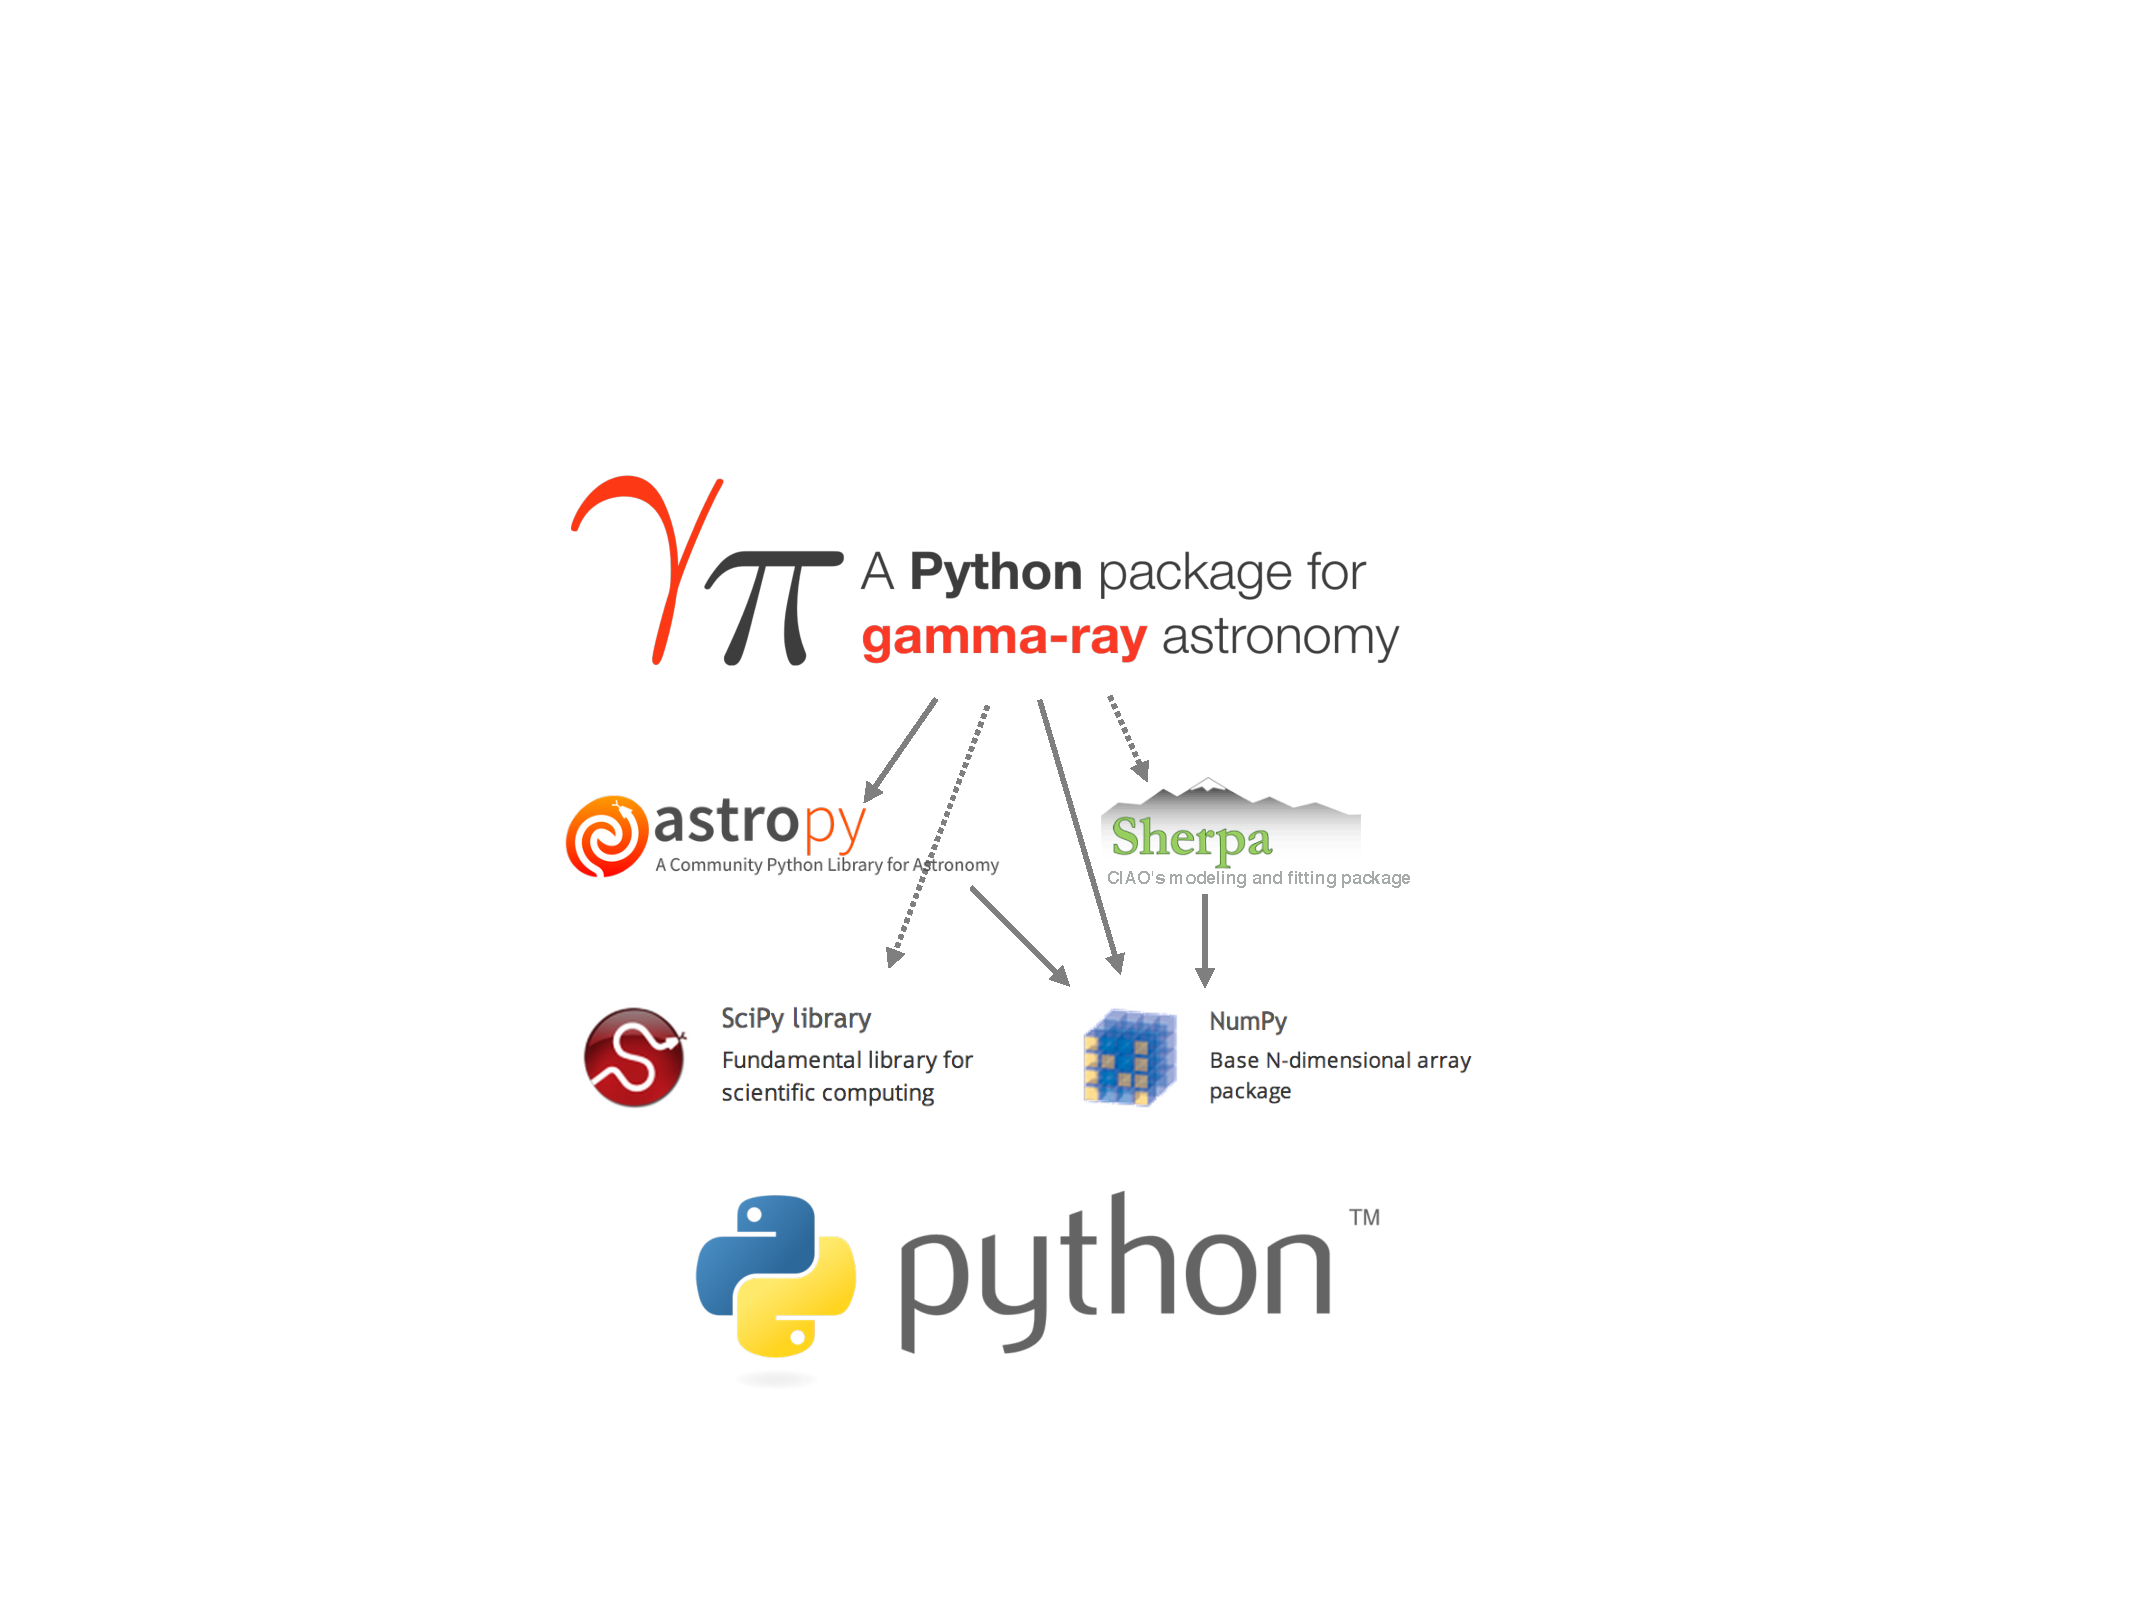
\includegraphics[width=0.7\textwidth]{figures/gammapy-stack}
\caption{
The Gammapy stack. Required dependencies Numpy and Astropy are illustrated with solid arrows, optional dependencies (the rest) with dashed arrows.
}
\label{fig:stack}
\end{figure}

\section{How Gammapy works: a code example}
\label{sec:code}

Gammapy is written high-level Python code, the data is stored in Numpy arrays or
objects such as {\it astropy.coordinates.SkyCoord} or {\it astropy.table.Table}
that hold Numpy array data members. Almost all functionality needed has been
written in C and Python wrappers already. Specifically, {\it astropy.wcs} is
calling into WCSLib (\cite{wcslib}), {it astropy.io.fits} uses CFITSIO
(\cite{cfitsio}) and {\it astropy.coordinates} as well as {\it astropy.time} are
built on ERFA (\url{https://github.com/liberfa/erfa}), the open-source variant
of this IAU Standards of Fundamental Astronomy (SOFA) C library
(\url{http://www.iausofa.org/}).

An example script that generates a counts image from an event list using Gammapy
is shown in Figure~\ref{fig:code_example}. The remarkable point we would like to
make here is that it is possible to efficiently work with events and pixels and
to implement algorithms from Python, by storing all data in Numpy arrays and
processing via calls into existing C extensions in Numpy and Astropy. E.g. here
{\it EventList} stores the RA and DEC columns from the event list as Numpy
arrays, and {\it SkyImage} the pixel data as well, and {\it image.fill(events)},
and all processing happens in existing C extensions (Numpy histograms and
Astropy calls into the CFITSIO and WCSLib C libraries). Should the need arise,
that some algorithm can't be efficiently implemented in pure Python, a small C
extension can be added to Gammapy, using e.g. Cython \cite{cython}.

We note that a huge eco-system of scientific Python packages that operate on Numpy arrays is available for advanced users, to implement analysis methods for special use cases (e.g. sky or background models, IRF handling or likelihood or Bayesian analysis methods). To name just a few that we have seen used in conjunction with Gammapy so far (by users, not within the Gammapy package itself): healpy, Scipy, pandas, scikit-image, scikit-learn, iminuit, emcee.

\begin{figure}[t]
\centering
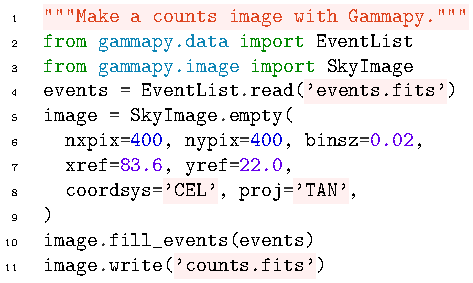
\includegraphics[width=0.5\textwidth]{examples/code_events_image}
\caption{
An example script using Gammapy to make a counts image from an event list. This
is used in Section~\ref{sec:code} to explain how Gammapy achieves efficient
processing of event and pixel data from Python: all data is stored in Numpy
arrays and passed to existing C extensions in Numpy and Astropy.
}
\label{fig:code_example}
\end{figure}

\section{Gammapy development}

Gammapy development happens on Github
(\url{https://github.com/gammapy/gammapy}). We make extensive use of the pull
request system to discuss and review code contributions. For testing we use
pytest (\url{https://pytest.org}), for continuous integration travis-ci (Linux
and Mac) as well as Appveyor (Windows). For documentation Sphinx
(\url{http://www.sphinx-doc.org}), for tutorial-style documentation Jupyter
notebooks (\url{https://jupyter.org/}) are used.

Gammapy is distributed and installed in the usual way for Python packages. Each
stable release is uploaded to the Python package index
(\url{https://pypi.python.org}), and downloaded and installed by users via {\it
pip install gammapy} (\url{https://pip.pypa.io}). Binary packages for conda are
available via the conda Astropy channel
(\url{https://anaconda.org/astropy/gammapy}) for Linux, Mac and Windows, which
conda users can install via {\it conda install gammapy -c astropy}. Binary
packages for the Macports package manager are also available, which users can
install via {\it port install gammapy}. Concerning Linux, at this time, Gammapy
is available as a Gentoo package
(\url{https://packages.gentoo.org/packages/dev-python/gammapy}) and a Debian
package is in preparation.

A public mailing list for Gammapy is available at
\url{https://groups.google.com/forum/\#!forum/gammapy} and for Gammapy developer
team communication we use Slack \url{gammapy.slack.com}. Two face-to-face
meetings for Gammapy were organized so far, the first on in June 2016 in
Heidelberg as a coding sprint for developers only, the second on in February
2017 in Paris as a workshop for both Gammapy users and developers.

Note that the current setup described in this section is different from what it
will be if Gammapy is chosen to be the or part of the CTA science tools, since
CTA will set up their own systems for software development, maintenance,
testing, documentation, issue tracking, software distribution and user support.

\section{Application example}
\label{sec:application}

In this poster we focused on the software and technical aspects of Gammapy. For
examples of CTA science studies using Gammapy, we refer you to other posters presented at this conference: Galactic survey \cite{roberta}, PeVatrons \cite{cyril} and extra-galactic sources \cite{julien}.

Several other examples using real data from H.E.S.S. and Fermi-LAT, as well as
simulated data for CTA can be found via \url{http://docs.gammapy.org} by
following the link to ``tutorial notebooks''. Figure~\ref{fig:app} shows one
result of the ``CTA data analysis with Gammapy'' notebook: a significance sky
image of the Galactic center region using 1.5~hours of simulated CTA data. The
background was estimated using the ring background estimation technique, and
peaks above 5~sigma are shows with white circles.

% \url{https://nbviewer.jupyter.org/github/gammapy/gammapy-extra/blob/master/notebooks/cta\_data\_analysis.ipynb}

\begin{figure}[t]
\centering
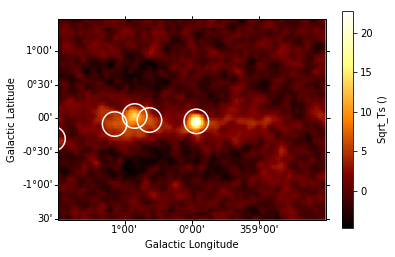
\includegraphics[width=0.7\textwidth]{figures/gammapy_example_sky_image.png}
\caption{
Application example: significance image for the Galactic centre region using 1.5~hours of simulated CTA data.  White circles are peaks above 5~sigma.
}
\label{fig:app}
\end{figure}

\section{Conclusions}
\label{sec:conclusions}

In the past two years, we have developed Gammapy as an open-source analysis
package for existing gamma-ray telescope and as a prototype for the CTA science
tools.

We find that the Gammapy approach, to build on the powerful and well-tested
Python packages Numpy and Astropy, brings large benefits: A small codebase that
is focused on gamma-ray astronomy in a single high-level language is easy to
understand and maintain. It is also easy to modify and extend as new use cases
arise, which is important for CTA, since it can be expected that the modeling of
the instrument, background and astrophysical emission, as well as the analysis
method in general (e.g. likelihood or Bayesian statistical methods) will evolve
and improve over the next decade. Last but not least, the Gammapy approach is
inherently collaborative, sharing development effort as well as know-how with
the larger astronomical community, that to a large degree already has adopted
Numpy and Astropy as the basis for astronomical analysis codes in the past 5
years.

\section{Acknowledgements}
\label{sed:acknowledgements}

This work was conducted in the context of the CTA Consortium. We gratefully
acknowledge financial support from the agencies and organizations listed here:
% TODO: the underscore doesn't work here -> not a link in the PDF. Why and how to fix?
\url{http://www.cta-observatory.org/consortium\_acknowledgments}

We would like to thank the Scientific Python and specifically the Astropy
community for providing their packages which are invaluable to the development
of Gammapy, as well as tools and help with package setup and continuous
integration, as well as building of conda packages.

We thank the GitHub (\url{http://www.github.com}) team for providing us with an
excellent free development platform, ReadTheDocs (\url{https://readthedocs.org})
for free documentation hosting, Travis (\url{https://www.travis-ci.org}) and
Appveyor (\url{https://appveyor.com}) for free continuous integration testing,
and Slack (\url{https://slack.com/}) for a free team communication channel.

\bibliography{gammapy-icrc2017}
\bibliographystyle{JHEP}

\end{document}
